\subsection{Komponentendiagramm zum Server}
\begin{figure}[H]
    \centering
    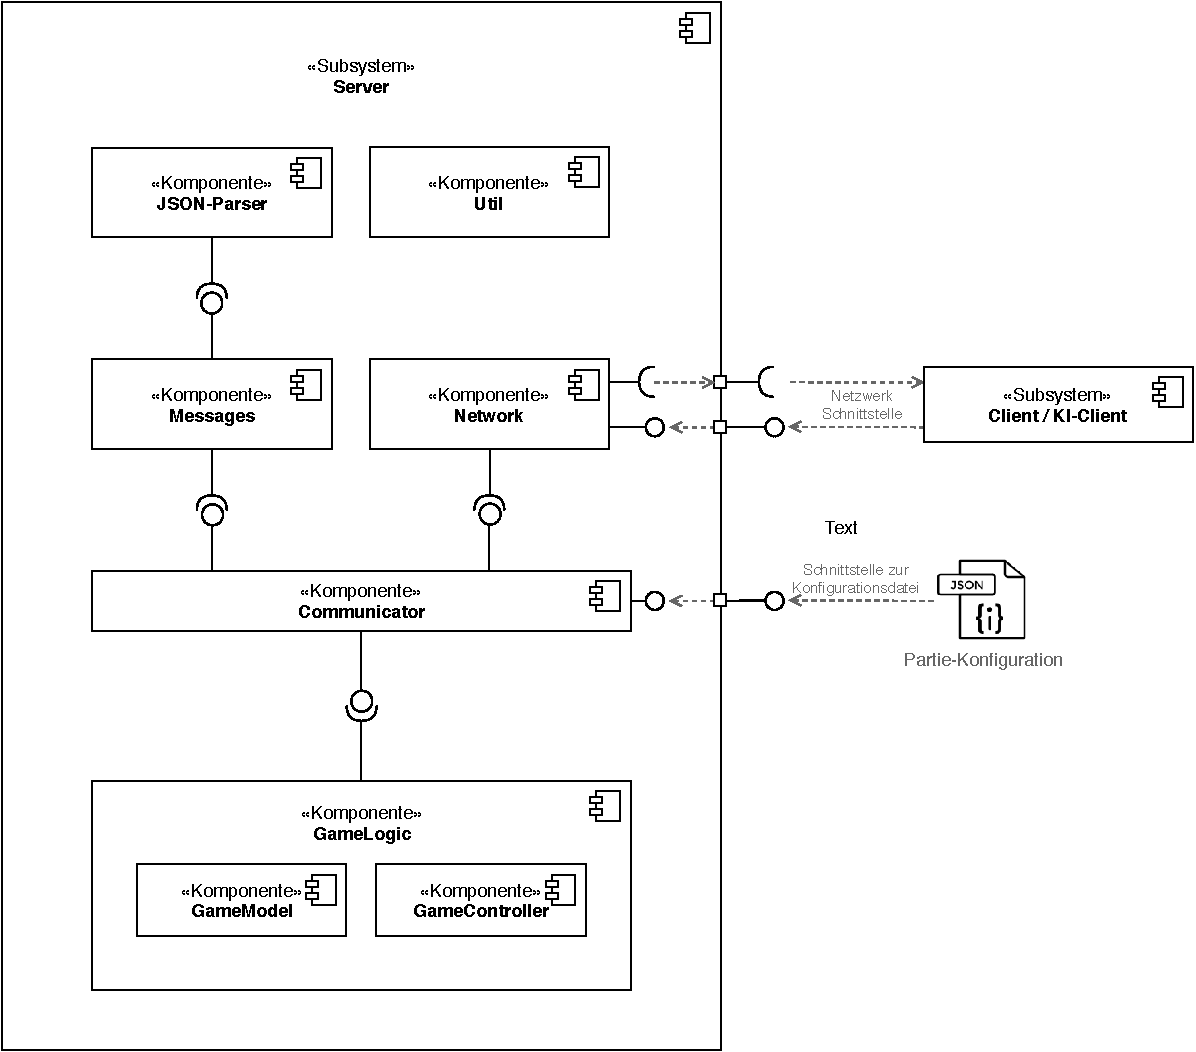
\includegraphics[scale=0.85]{../Endabnahme/images/ServerDiagramme.pdf}
\end{figure}
Die Serveranwendung lässt sich grob in zwei Teile aufteilen: Die Spiellogik und den Kommunikator. Der Kommunikator ist für das Senden und Empfangen von Nachrichten, sowie für das Verwalten von Verbindungen und mehreren Lobbys zuständig. Empfangene Nachrichten werden an die Spiellogik weitergeleitet, die so den internen Spielzustand aktualisieren kann. Diese Updates werden dann wieder über den Kommunikator an die Clients verteilt. Diese Aufteilung ermöglicht es uns, die einzelenen Komponenten bei der KI wiederzuverwenden. Die Komponenten sind voneinander komplett unabhängig und können deswegen einfacher getestet und verändert werden.

Genauer betrachtet, sind die zwei Hauptkomponenten weiter unterteilt. Die Spiellogik besteht aus GameModel und GameController. Erstere repräsentiert ausschließlich einen kompletten Spielzustand, ohne Informationen über die aktuelle Phase oder Ähnliches. Ein so repräsentierter Spielzustand lässt sich durch Methoden im GameController in einen anderen konsistenten Spielzustand überführen. Auch hier dient die Modularität der besseren Test- uns Wartbarkeit.

Der Kommunikator nutzt intern die Messages- und Network-Bibliotheken. Erstere implementiert alle verschiedenen Nachrichtentypen, zweitere ist ein moderner C++-Wrapper für die in C geschriebene libwebsockets-Bibliothek.

Zu guter Letzt werden allgemeine Tools wie z.B. ein Logging-Mechanismus oder Timer von unserer Utils-Bibliothek zur Verfügung gestellt.

\subsection{Komponentendiagramm zur KI}
\begin{figure}[H]
    \centering
    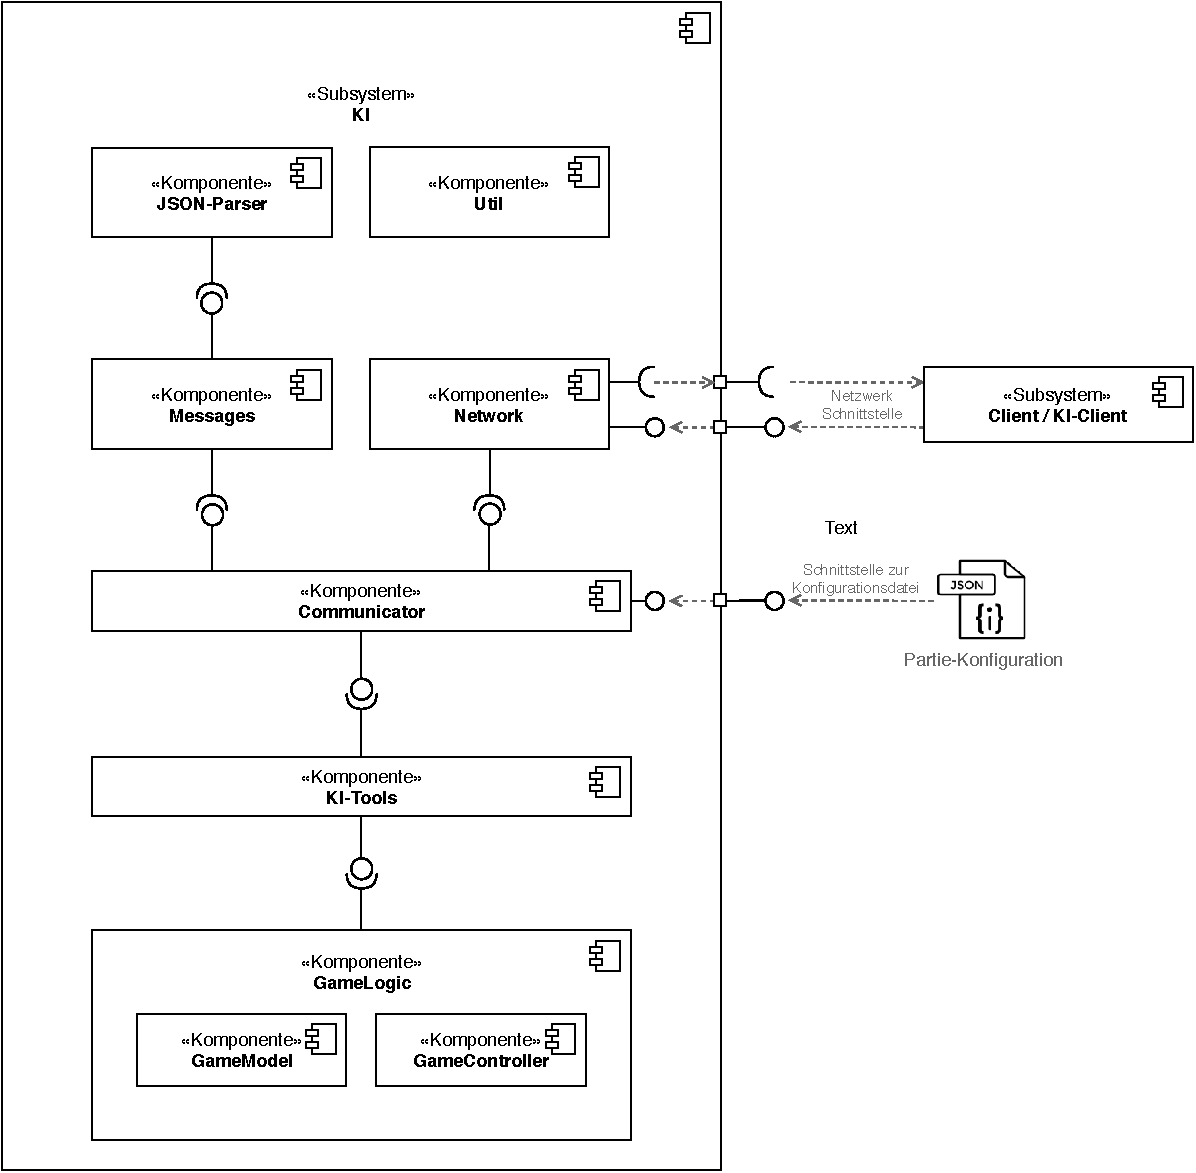
\includegraphics[scale=0.85]{../Endabnahme/images/KiDiagramme.pdf}
\end{figure}
Durch die bereits bei der Serverkomponente angesprochenen Vorteile ist die KI fast identische zum Server aufgebaut. Der einzige Unterschied ist, dass die KI selbstständig Züge ausführen muss. Dazu verwendet sie Methoden aus der AI-Toolbox wie beispielweise Such- und Optimierungsalgorithmen.

\subsection{Komponentendiagramm zum Benutzer-Client}
\begin{figure}[H]
    \centering
    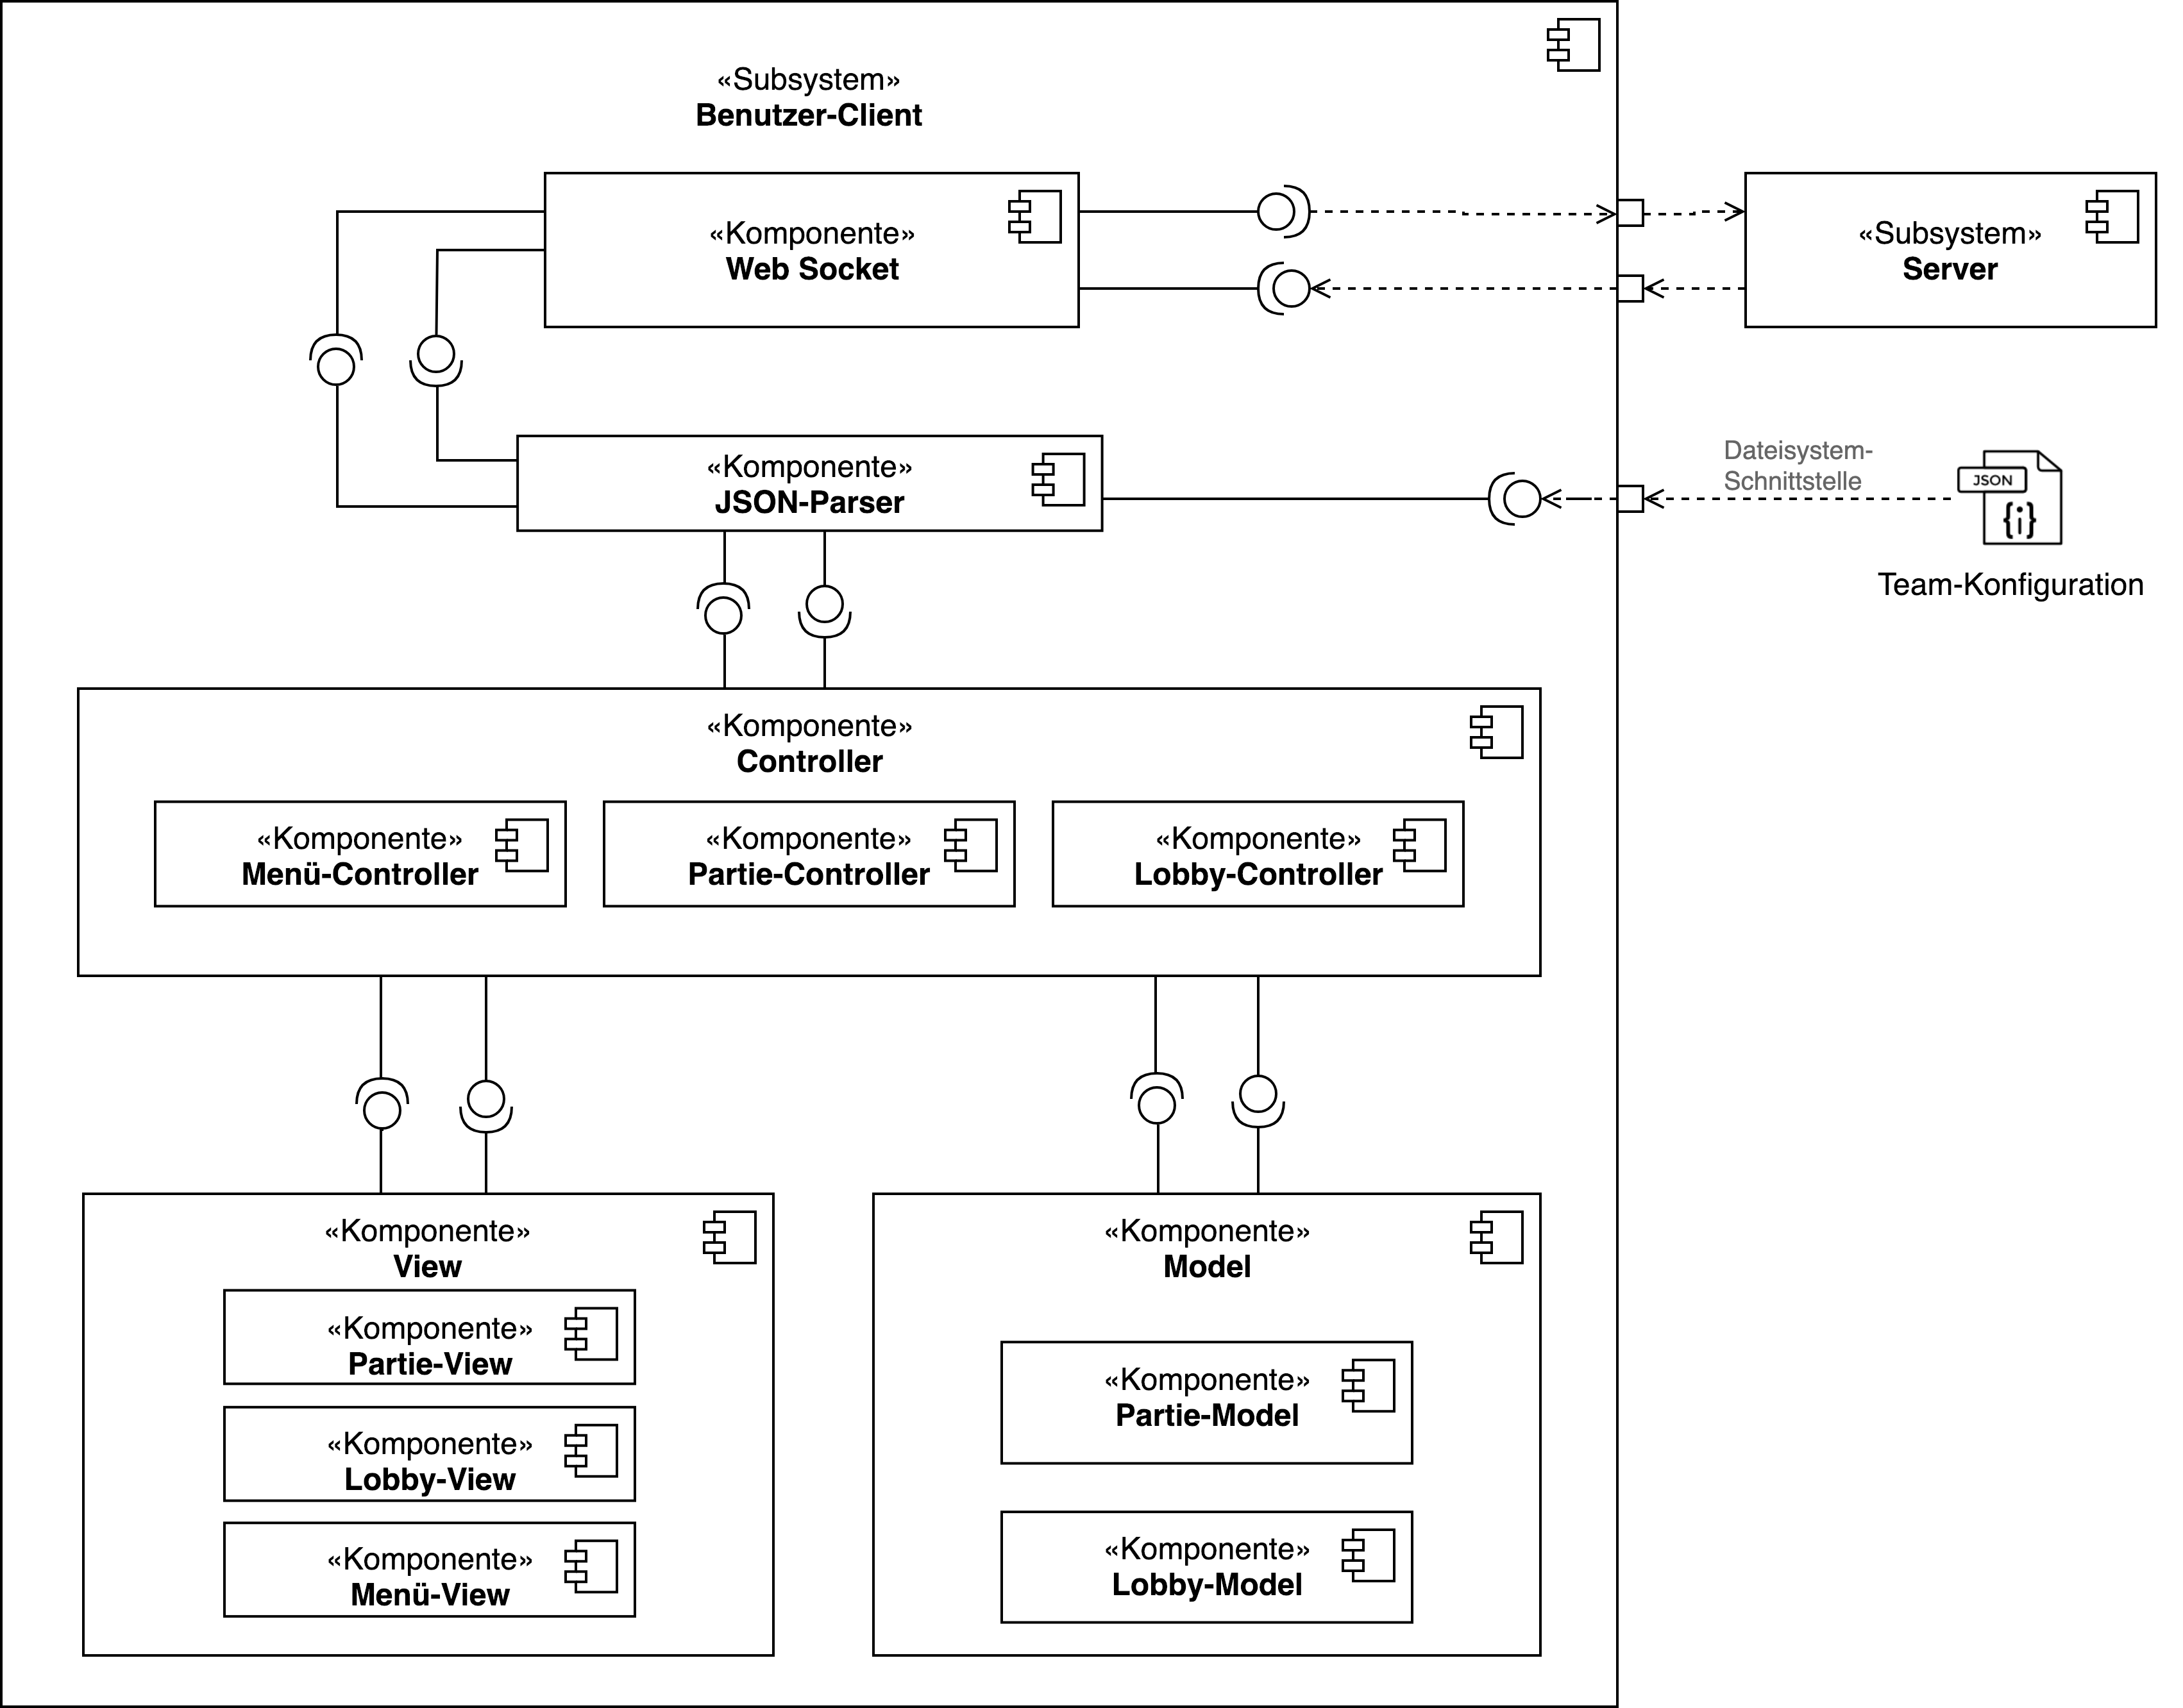
\includegraphics[scale=0.13]{../Meilenstein05/images/komponentendiagramm_benutzer-client.png}
\end{figure}
Der Client ist nach dem MVC-Prinzip aufgebaut. Für die verschiedenen Ansichten gibt jeweils eine View. Im Model werden die aktuelle Spielzustände bzw. Daten für den Anmeldevorgang gespeichert. Der Controller kommuniziert sowohl mit Model und View, als auch mit der Netzwerkschnittstelle.


\subsection{Komponentendiagramm zum Level-Editor}
\begin{figure}[H]
    \centering
    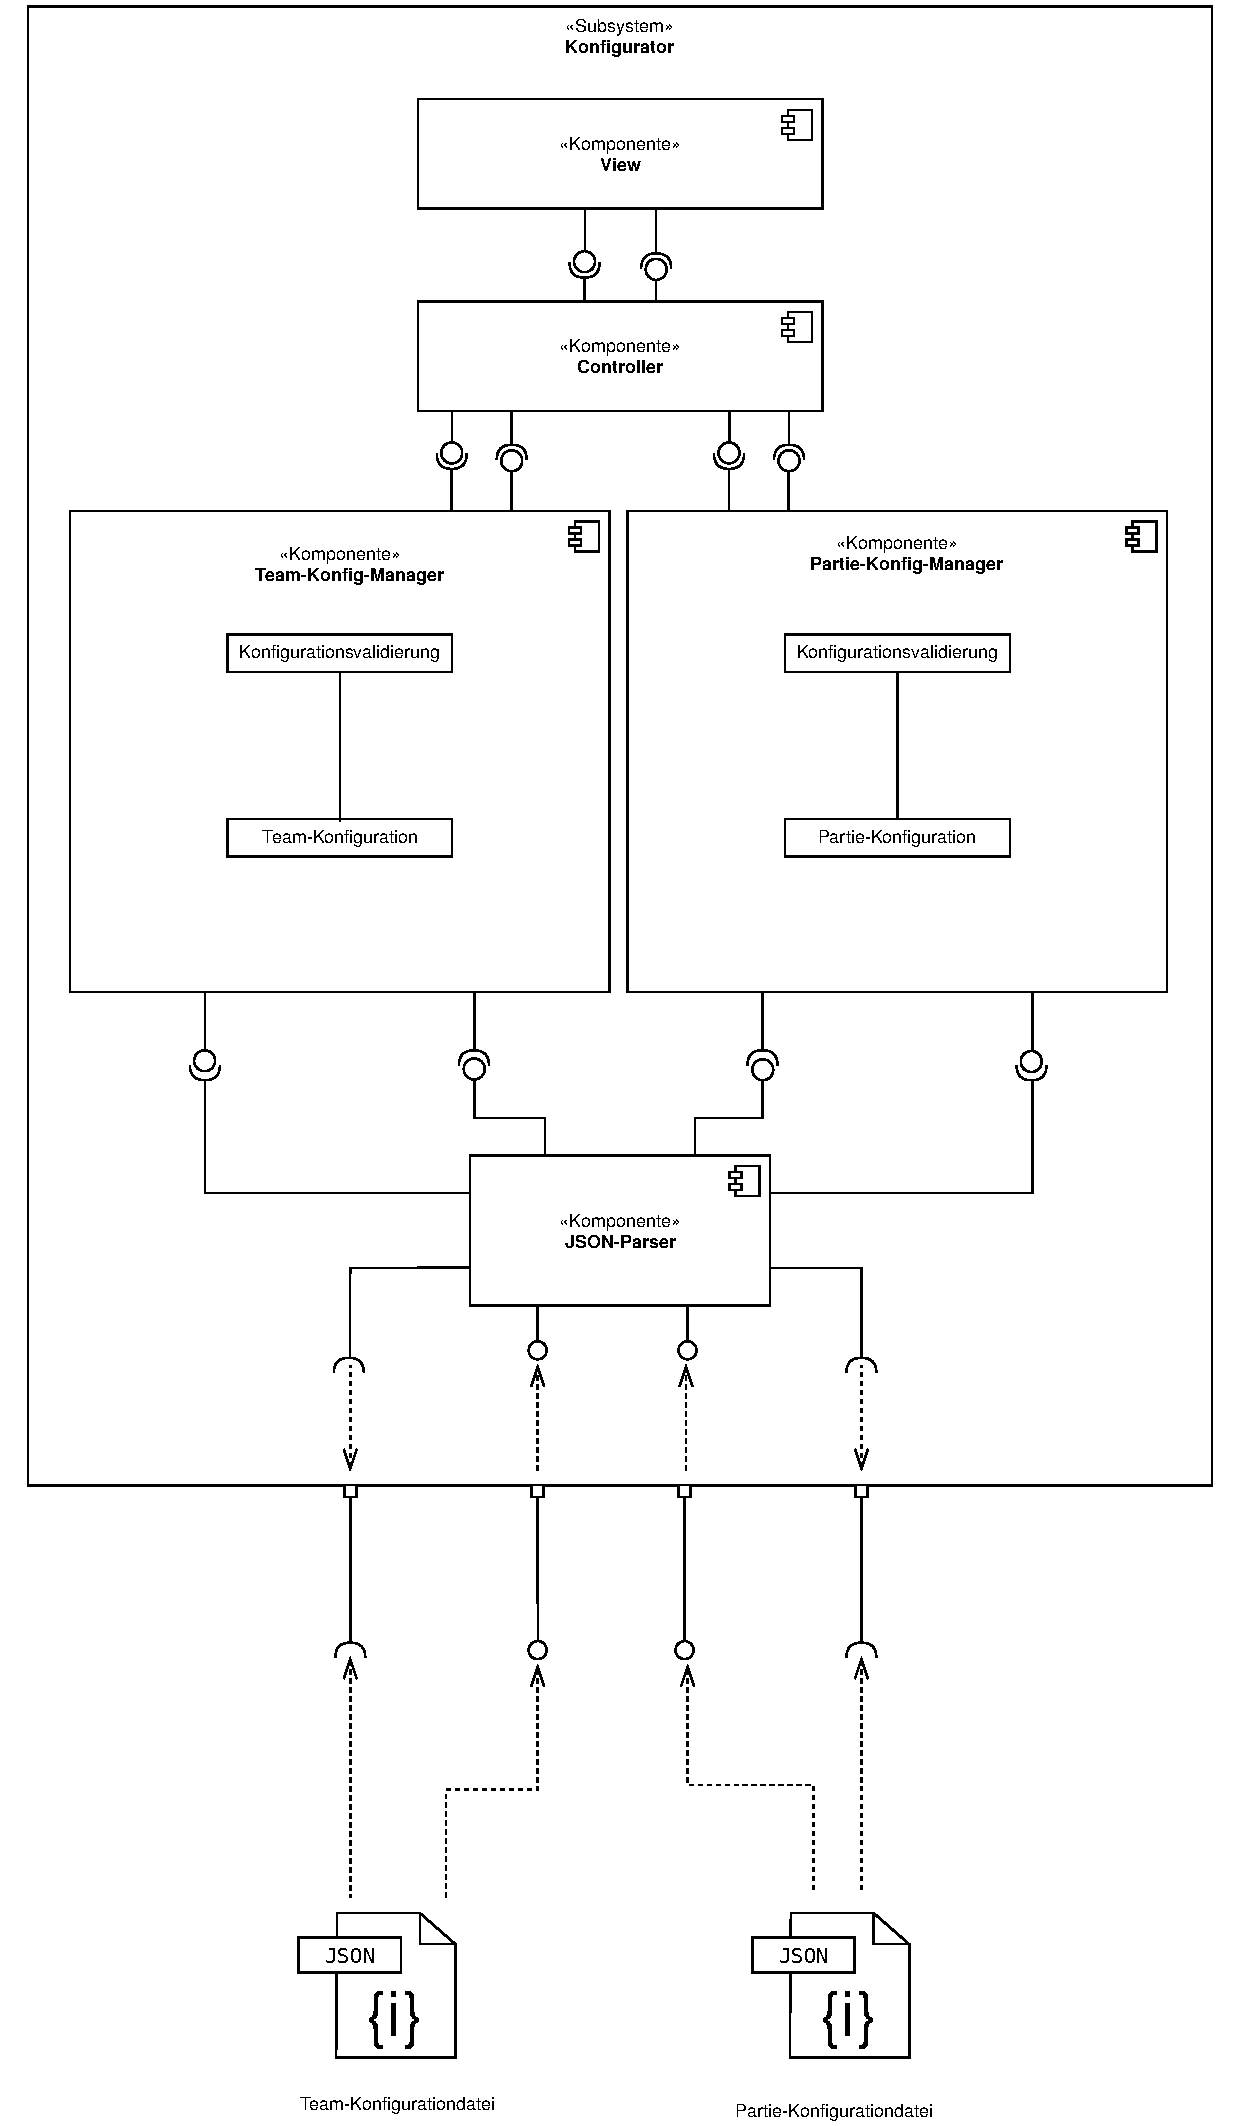
\includegraphics[scale=0.5]{../Meilenstein05/images/Konfigurator.pdf}
\end{figure}
Wie auch der eigentliche Client ist der Konfigurator nach dem MVC-Prinzip aufgebaut.
